% !TeX root = ./seminararbeit.tex
%% Preambel
\documentclass[conference,compsoc,final,a4paper]{IEEEtran}
\usepackage[utf8]{inputenx}

%% Bitte legen Sie hier den Titel und den Autor der Arbeit fest
\newcommand{\autoren}[0]{Mundhenke, Moritz}
\newcommand{\dokumententitel}[0]{Spectre and Cloud : An evaluation of threats in shared computation environments }

% Hie muss normalerweise nichts angepasst werden
\usepackage[pdftex]{graphicx}
\graphicspath{{img/}}
\DeclareGraphicsExtensions{.pdf,.jpeg,.jpg,.png}
\usepackage[cmex10]{amsmath}
\usepackage{algorithmic}
\usepackage{array}
\usepackage{dblfloatfix}
\usepackage{url}
\usepackage[autostyle=true]{csquotes}
\usepackage[backend=biber]{biblatex}
\usepackage{booktabs}
\usepackage{xcolor}
\usepackage{listings}             % Source Code listings
\usepackage[printonlyused]{acronym}
\usepackage{fancyvrb}

% Farben definieren
\definecolor{linkblue}{RGB}{0, 0, 100}
\definecolor{linkblack}{RGB}{0, 0, 0}
\definecolor{darkgreen}{RGB}{14, 144, 102}
\definecolor{darkblue}{RGB}{0,0,168}
\definecolor{darkred}{RGB}{128,0,0}
\definecolor{comment}{RGB}{63, 127, 95}
\definecolor{javadoccomment}{RGB}{63, 95, 191}
\definecolor{keyword}{RGB}{108, 0, 67}
\definecolor{type}{RGB}{0, 0, 0}
\definecolor{method}{RGB}{0, 0, 0}
\definecolor{variable}{RGB}{0, 0, 0}
\definecolor{literal}{RGB}{31,0, 255}
\definecolor{operator}{RGB}{0, 0, 0}

\usepackage[english]{betababel}
\usepackage[
      unicode=true,
      hypertexnames=false,
      colorlinks=true,
      colorlinks=false,
      linkcolor=darkblue,
      citecolor=darkblue,
      urlcolor=darkblue,
      pdftex
   ]{hyperref}
%	 \PrerenderUnicode{ü}

% Einstellungen für Quelltexte
\lstset{
    xleftmargin=0.1cm,
    basicstyle=\scriptsize\ttfamily,
    keywordstyle=\color{keyword},
    identifierstyle=\color{variable},
    commentstyle=\color{comment},
    stringstyle=\color{literal},
    tabsize=2,
    lineskip={2pt},
    columns=flexible,
    inputencoding=utf8,
    captionpos=b,
    breakautoindent=true,
    breakindent=2em,
    breaklines=true,
    prebreak=,
    postbreak=,
    numbers=none,
    numberstyle=\tiny,
    showspaces=false,      % Keine Leerzeichensymbole
    showtabs=false,        % Keine Tabsymbole
    showstringspaces=false,% Leerzeichen in Strings
    morecomment=[s][\color{javadoccomment}]{/**}{*/},
    literate={Ö}{{\"O}}1 {Ä}{{\"A}}1 {Ü}{{\"U}}1 {ß}{{\ss}}2 {ü}{{\"u}}1 {ä}{{\"a}}1 {ö}{{\"o}}1
}

\hypersetup{
    pdftitle={\dokumententitel},
    pdfauthor={\autoren},
    pdfdisplaydoctitle=true,
    hidelinks
}

% Makros für typographisch korrekte Abkürzungen
\newcommand{\zb}[0]{z.\,B.\ }
\newcommand{\dahe}[0]{d.\,h.\ }
\newcommand{\ua}[0]{u.\,a.\ }

% Wo liegt Sourcecode?
\newcommand{\srcloc}{src/}

% Literatur einbinden
\addbibresource{literatur.bib}
 % Weitere Einstellungen aus einer anderen Datei lesen

\begin{document}

% Titel des Dokuments
\title{\dokumententitel}

% Namen der Autoren
\author{
  \IEEEauthorblockN{\autoren}
  \IEEEauthorblockA{
    Mannheim University of Applied Sciences\\
    Department of Computer Science\\
    Paul-Wittsack-Str. 10,
    68163 Mannheim
    }
}

% Titel erzeugen
\maketitle
\thispagestyle{plain}
\pagestyle{plain}

% Eigentliches Dokument beginnt hier
% ----------------------------------------------------------------------------------------------------------

% Kurze Zusammenfassung des Dokuments
\begin{abstract}
The processor flaws used in the Spectre and Meltdown attacks have had uncharacteristically large media impact even gaining coverage in main stream media. This is despite the fact that this type of exploit has not been used in any real attacks and is unlikely to target consumers, as simpler attack vectors still remain highly effective. However, because Spectre affects any processor which uses speculative execution with little hope for a \enquote{silver bullet} in the near future, Spectre seems to be here to stay. \\
While Spectre might not very relevant to the consumer market, it is quite relevant where safety is usually paramount. The cloud promises cost reduction and safety through offloading maintenance and updating to gigantic providers like Amazons AWS. But how secure can the most up-to-date platform be if the used hardware is inherently flawed to the core? \\
This paper shows potential attack vectors in a shared cloud environment, discusses some defensive measures and provides a high level explanation of the Spectre attack.
\end{abstract}

% Inhaltsverzeichnis erzeugen
\tableofcontents

% Abschnitte mit \section, Unterabschnitte mit \subsection und
% Unterunterabschnitte mit \subsubsection
% -------------------------------------------------------
\section{Introduction}
Cloud computing can offer enormous cost savings by reducing administrative effort for the customer and make use of hardware more efficiently by maximizing utilization. To achieve this increased utilization, hardware has to be shared in some form between multiple customers. In combination with the hardware flaws uncovered by the Spectre attacks and the potential for anyone to buy cloud resources, this creates an entirely new threat model for cloud applications. \\
To investigate this problem we first discuss the technologies used in todays computation environment that play a part in Spectre attacks. Afterwards compute cloud offerings are differentiated and potential attack vectors shown. This is done through a combination of past attacks on cloud infrastructure and potential application of Spectre exploits in these scenarios to determine the associated risks. These risk remain entirely theoretical as experimental proof of such attacks is outside of the scope of this work. \\
Finally mitigation options are discussed and some recommendations based on the findings of this work are given.

% -------------------------------------------------------
\section{Modern computation hardware and infrastructure}
\subsection{Memory management}
\begin{figure}[!ht]
\centering
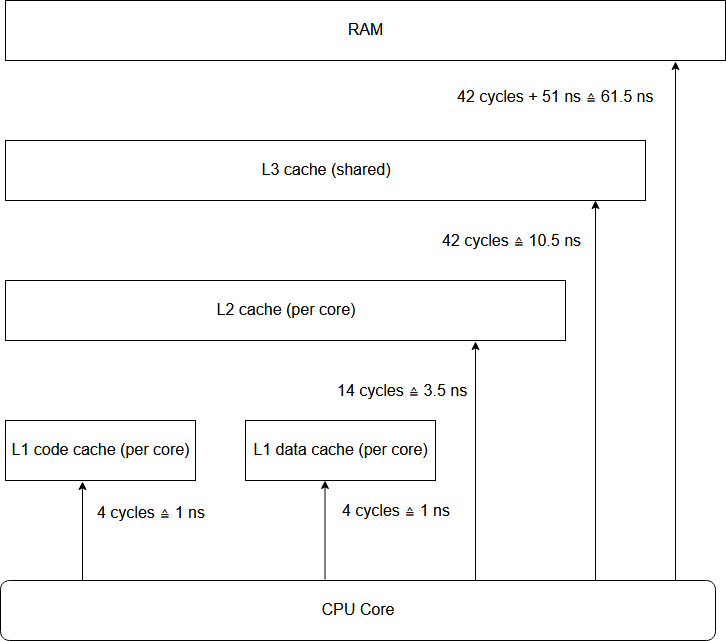
\includegraphics[width=8.5cm]{caches.png}
\caption{The Intel Skylake cache hierarchy and access latencies\cite{fog2012microarchitecture}. Timings are calculated assuming a clock speed of 4 GHz for an Intel i7-6700 processor using DDR4-2400 RAM\cite{skylakeBenchmark}. }
\label{caches}
\end{figure}
Since around 1980 memory performance has not been able to keep up with the ever increasing processor speeds. \cite[p.~73]{hennessy2011computer} Because of this accessing the main memory has become a very time consuming task. Modern processors therefore try to circumvent RAM access through the use of multiple cache layers (see. \autoref{caches}). These caches have a rather limited capacity especially the very fast L1 cache (Skylake i7-6700 L1 cache 2x32KB per core, L3 cache 8MB total). \cite{skylakeBenchmark} \\
To optimize the usage of the available caches, various techniques are used. When code access a memory address, such as an array or string, it is very likely that addresses nearby will also be accessed (\emph{spatial locality}). Because of this memory is loaded into the caches in blocks to reduce cache misses in these cases. \cite[p.~74]{hennessy2011computer}. \\

\subsection{Processor pipelines and speculative execution}
Since the turn of the millennium, clock speeds of high performance CPU's have stagnated because the increased energy consumption and resulting heat generation got
too high. \cite{fog2012microarchitecture} Multi-core architectures became common however even today many, if not most,
workloads rely heavily on single thread performance. Therefore, to increase the speed of single thread execution, without increasing the clock speed,
more instructions have to be executed in a single cycle. To achieve this goal many techniques like instruction splitting, fusion,
and simultaneous instruction execution are used. \cite{fog2012microarchitecture} These optimizations require more complex processing of the instruction stream which
is handled by the processors instruction pipeline. This has resulted in higher pipeline memory requirements as well as a longer pipelines in terms of clock cycles
required for an instruction to complete execution. However, since programs use conditional branches and loops these long pipeline can become invalid because the CPU
cannot know the destination of a conditional jump without first evaluating the condition. This results in a pipeline flush that wastes valuable execution time while
the pipeline is refilled. To mitigate the impact of this issue the processor can store previous outcomes of branches and use this to predict future executions of the
branch. With branch prediction only a miss-prediction will result in a pipeline flush. The CPU runs the instruction of the predicted branch and either commits
the results if the prediction was correct or discards them if was not.
This process is called speculative execution. \cite{kocher2018spectre}
\subsection{Virtual and shared memory}
\begin{figure}[!ht]
\centering
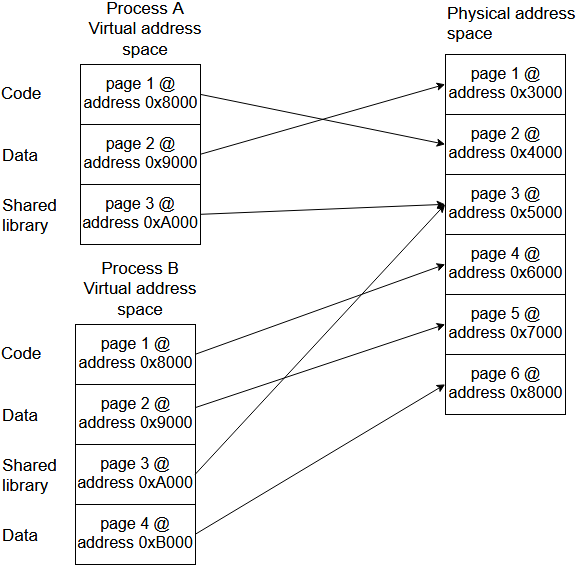
\includegraphics[width=8.5cm]{virtMem.png}
\caption{Mapping of virtual memory to physical memory. }
\label{virtmem}
\end{figure}
Running multiple programs in parallel is a operating system \enquote{feature} that has been the standard for around 30 years. Before that some operating systems would run only one program at a time or completely swap out the main memory when switching to a different running process. \cite{tanenbaum1997operating} This method is obviously not very efficient and handling many processes at once. Today, virtual memory is the primary way of managing memory. When using virtual memory every process has it own separate address space. This means two processes can store different data at the same address without being able to affect each other. \cite[p.~620]{hennessy2011computer}\\
The virtual address space of each process is divided into memory blocks called pages (currently on x86 computers page size is 4kB). When a process accesses an address the virtual page address is translated by the \ac{MMU} to a physical page address or, when the page is not loaded into memory, gets loaded into memory by the OS. \\
While virtual memory allows reuse of the same virtual address by multiple processes, it also allows sharing of physical memory between processes. This can be used for inter process communication and also as an optimization to share identical code between programs. Shared libraries are loaded once and can be reused by any program that uses the same library version. \cite{tanenbaum1997operating} To prevent programs from changing the library code for other programs, a copy on write mechanism is used. When a process attempts to write to a shared library page, it is copied in physical memory and the virtual address gets remapped to the copied version.
\subsection{Docker}
\subsubsection*{Containerization concept}
Docker allows isolation of processes in containers. These containers hide other processes running on the host and provide the process with its own virtual filesystem
and network. This means containers only share the hosts kernel which stands in contrast with classical VMs which have to run a separate OS for
each virtual machine. \cite{bernstein2014containers}\\
To create a container an image is used. The image contains all required files and serves as a \enquote{blueprint} for the container. \cite{bernstein2014containers}
Due to the lightweight nature of containers it is possible and best practice to isolate every application in its own container. \cite{dockerBestPractices} For example a
classic PHP and MySQL application, also called LAMP stack (Linux, Apache, MySQL and PHP), would use a MySQL and an Apache container. This has multiple benefits:
Developers can build and test container images on their own machine which will behave identical when run on a production server. Docker also allows easy horizontal
scaling of applications. The LAMP stack mentioned above could be extended by creating an additional Apache container and an nginx container
to load balance between the two Apache servers.
\subsubsection*{File-system layers}
To reduce redundancy docker images are divided into layers. \cite{dockerBestPractices} For example an Apache PHP application would consist of 3
major layers. The first contains a minimal debian image providing basic libraries and tools. The second layer contains Apache and its dependencies. The final
layer would then have a copy of the applications PHP source files. \\
When a container is started from this image, the layers are stacked on top of each other
using a union filesystem like OverlayFS\cite{overlayfs}. Whenever the application attempts to read a file, the kernel checks each layer from top to bottom
returning the first result. This allows overriding of files on lower layers. \\
Because of this multiple different PHP images can share the first two layers and a MySQL image
sharing the base Debian image. Docker also adds a final non-persistent layer to the container which the application running inside uses to write files,
which is discarded when the container is shutdown.
\subsection{Cloud}
NIST defines cloud computing as \enquote{\textelp{} a model for enabling ubiquitous, convenient, on-demand network access to a shared pool of configurable computing resources (e.g., networks, servers, storage, applications, and services) that can be rapidly provisioned and released with minimal management effort or service provider interaction.} \textcite{mell2011nist}. Further more 5 essential characteristics are defined: On-demand self-service, broad network access, resource pooling, rapid   elasticity and measured service. Resource pooling is of special interest in the context of this work. \\
Cloud resources are shared by multiple costumers in a multi-tenant model. \cite{mell2011nist} Concretely this means that tenants(customers) of a cloud platform share a server provided by the platform. This might be in form of quite direct sharing of a server by running virtual machines owned by different tenants on it. However, more abstract offerings like \ac{SaaS} databases which give the customer no direct control over an operating system will have some form of resource sharing. \\
This results in customers having to trust not only the confidentiality of the provider itself, but also trust the isolation that separates them from potentially malicious third parties.
% -------------------------------------------------------
\section{Spectre}
\subsection{Side-channels}
Computer programs can, on an abstract level, be described with the \ac{IPO} model. An input will produce an output defined by the algorithms
of the program. This output is deterministic, meaning input \lstinline|a| will always result in output \lstinline|b|. \\
However, in real life systems, processes can produce additional outputs which are not intended by its programmer. For example a program which calculates the
factorial of a number takes longer proportional to the input number. An attacker could therefore, infer the input number from the execution time without knowing the
result. More complex timing-attacks have been used to extract private keys or other secrets
of various cryptographic algorithms. \cite{bernstein2005cache}\cite{kocher1996timing}
Similarly even a systems power consumption can be used as a side-channel to retrieve secret data. \cite{kocher1999differential} \\
While these two side-channels can add unintended output to a process they are within the programmers control. Execution time can be increased arbitrarily through
idling or sleeping and the system's power consumption can be increased by running pointless code. Other side-channels however, are completely outside of the
control of the programmer. For example a program has very limited or no direct control over the systems cache state or which \ac{ALU} will compute a calculation.
\subsection{Exploiting speculative execution}
To execute a spectre exploit the attacker first has to find a vulnerable instruction sequence in the victim program. The sequence will leak secret data into the chosen
side-channel during speculative execution. Therefore, spectre-style attacks can be differentiated from each other by the how speculative execution is achieved
and what side-channel is used. \cite{kocher2018spectre} \\
The example of Variant 1 of the original spectre attack uses conditional branches to achieve speculative
execution and leaks data through the processors cache state. The conditional branch is an array bounds check \lstinline|if (x < array1_size)|. The branch prediction
can be miss-trained by repeatedly calling the victim function with an in-bounds \lstinline|x| causing it to predict the branch as true in the future. Then the
attacker flushes \lstinline|array1_size| from the processors cache and calls the victim function again. This causes the branch to be execute speculatively
until \lstinline|array1_size| is retrieved from memory. \\
To leak the victims secret the attacker chooses an \lstinline|x| that is out of bounds. The victim
now reads from \lstinline|array1| using the malicious, out-of-bounds address. To successfully execute the attack sequence the victim also has to use the result to
access a second array. This causes the processor to load a memory address into the cache which is based of the previous out-of-bounds access of \lstinline|array[x]|.
The attacker can now time their own access of the possible memory addresses, revealing which address can be read fastest and was therefore retrieved by the victims
speculative execution, revealing the (secret) value of \lstinline|array[x]|.
% -------------------------------------------------------
\section{Spectre in shared cloud infrastructure}
\begin{figure}[!ht]
\centering
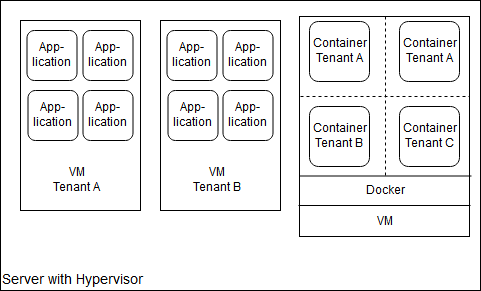
\includegraphics[width=8.5cm]{vmAndDocker.png}
\caption{Tenant isolation in a cloud environment using a hypervisor and using Docker container isolation.}
\label{virtmem}
\end{figure}
\subsection{Shared hypervisor}
\ac{IaaS} providers give their customers, here referred to as tenants, the ability to rent virtual machines. The tenant has full access
to this VM (root access). Since most applications do not require the full capabilities of the physical server, multiple VMs are run on a hypervisor such as VMware
ESXi or Linux's KVM. \\
This results in the sharing of physical resources like RAM and CPU cores between tenants. This isolation is hardware enforced
and hypervisor exploits are quite rare (only 5 ESXi vulnerabilities in 2018 with a score $\ge$ 5) \cite{esxiVulnerabilities}. However, since speculative execution can
circumvent hardware enforced checks, some Spectre vulnerabilities allowed an attacker to read the memory of another tenants VMs and the hypervisor
itself \cite{vmwareSpectre, vmwareSpectreNG}. While the currently known Spectre attacks have been mitigated by hypervisor patches, speculative execution exploits
found in the future could still allow cross VM attacks in the cloud. \\
In a public cloud an adversary is faced with another hurdle besides VM isolation. Because the \ac{IaaS} provider allocates resources for the tenants based on the their
requirements through a closed-source algorithm, an attacker can not directly force co-residency (share a hypervisor) with the victim. \\
\textcite{Ristenpart:2009:HYG:1653662.1653687} demonstrated various networking based techniques to achieve co-residency in the early (2009) \ac{AWS} cloud and while Amazon
has improved security in this regard, other co-residency detection mechanisms have been found \cite{inci2015seriously}. This newer method uses information leaks
on the processor level, specifically through the last level cache shared between all CPU cores.
\subsection{Shared Docker host}
Running docker containers in the cloud can have benefits for both the customer and the cloud provider. The customer does not have to worry about maintenance
of the underlying operating system and can more easily scale their application. The cloud provider can, in theory, increase utilization of their hardware
because of the reduced overhead. \\
However, leveraging these benefits requires faith in the process isolation provided by Docker and the Linux kernel. Because of this the Azure and \ac{AWS} public
cloud isolate containers using hypervisor technology, only sharing kernels between containers of the same user defined application group
\cite{fargateIsolation, azureIsolation}. Due to this the
potential price advantage is lost. The smallest possible \ac{AWS} Fargate task configuration (0.25 vCPU and 0.5 GB RAM) costs 0.01234 USD per hour\cite{fargatePricing}
while the EC2 t3.micro VM (2 vCPU and 1 GB RAM) only costs 0.0104 USD per hour \cite{ec2Pricing}. \\
Other \ac{PaaS} providers like
Heroku\cite{herokuIsolation}, OpenShift\cite{openshiftIsolation} and the defunct DotCloud however, do not use the additional isolation provided
by hypervisor virtualization\cite{zhang2014cross}. \\
These providers do refer to various \enquote{Docker hardening} techniques, however, specifics like the usage of
shared libraries between containers are not mentioned, which can provide attack surface area for Spectre exploits. \cite{retpolineTurner}
\subsection{\acs{FaaS} -- Function as a Service}
\begin{figure}[!ht]
\centering
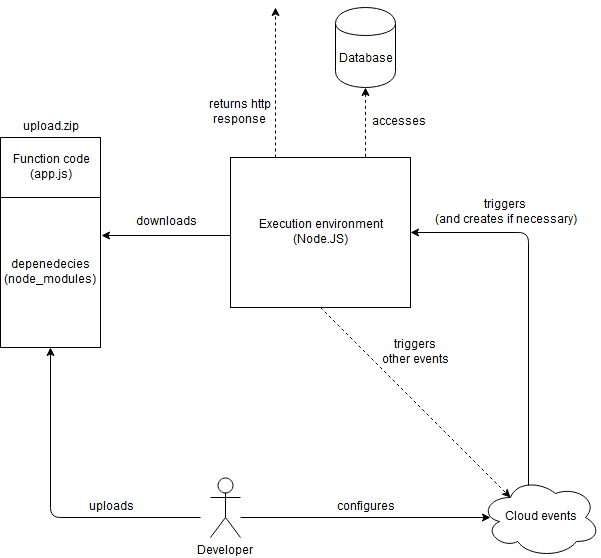
\includegraphics[width=8.5cm]{FaaS.png}
\caption{\ac{FaaS} example for a Node.JS application.}
\label{virtmem}
\end{figure}
\acs{FaaS} further abstracts service infrastructure. Conceptually a developer writes a function, uploads it to the \acs{FaaS} service and connects events like HTTP requests or
database events as an input source. \\
When an event occurs the function is called with the event's parameters and, in the case of an HTTP request, builds and
returns a API response. The benefits are automatic scaling and a payment model where the customer only pays for the functions execution time. \cite{lambdaFeatures}\\
In reality a \enquote{function} is a package of code, configuration and module/library files. Therefore, even if the service for example only allows Node.JS execution
this cannot be considered a security feature as a node module can contain native, compiled binary files. \cite{lambdaFaq} \\
Due to the high abstraction level, internal implementation details are sparsely documented. \ac{AWS} Lambda notes that Lambda functions are isolated using EC2 techniques, i.e.
hypervisor isolation\cite{lambdaFaq}. \ac{GCF} in contrast only states that functions are run in
\enquote{its own isolated secure execution context}\cite{cloudFunc}. \textcite{wang2018peeking} further investigates \acs{FaaS} implementations. \\
If a \acs{FaaS} would only use docker to isolate functions of different customers, the risk of a speculative attack would be higher compared to a Docker \ac{PaaS} provider. Since function are based on small number of available runtime environments (e.g.\ \ac{GCF}: Go, Python and Node.js 6,8,10) \cite{cloudFunc} an attacker has implicit knowledge
about the victims shared library and executable files. \\
Therefore, an attacker could not only attempt co-residency to gain access to a specific target's secrets, but instead mount a broader attack acquiring data from random
other tenants. Similar to spam phishing emails the goal would not be one large \enquote{heist} but instead gaining value from many smaller thefts.
% -------------------------------------------------------
\section{Prevention and detection}
\subsection{Hardware, Software and Compiler}
While meltdown could be mitigate by operating system patches \cite{linuxKAISER}, the spectre vulnerabilities have required cooperative changes to hardware, compilers and vulnerable software itself. \\
On the hardware side, some vulnerabilities have been removed in newer processors, others can be circumvented through new instructions that allow explicit prevention of speculative execution. \cite{intelMitigation} \\
Compilers have been adapted to reduce the generation of code blocks that are vulnerable to some forms of spectre attack \cite{msvcQSpectre} and insert code that traps speculative execution in an endless loop \cite{retpolineTurner}. \\
All of these changes require recompilation of programs, libraries, operating systems and drivers. Additionally all of these mitigation have some form of performance drawback and are therefore not enabled by default.
\subsection{In-memory encryption}
To prevent a Spectre attack from accessing secret data, the data could be encrypted in-memory. This technique however, has two weaknesses. The first issue arises from the
fact that to make use of the encrypted data the process has to, albeit briefly, decrypt the data. This results in the data still being vulnerable, but reduces an attacker's
window of opportunity to access the secret. \\
The second issue stems from encryption key storage. Since the key itself has to be stored in-memory for encryption/decryption it could be stolen together with the
encrypted data. \\
In a shared kernel environment, e.g.\  Docker, the key can be hidden completely from the attacker by storing it outside of the victims address space. This is due to
the limitation of Spectre, that an attack can only access memory the victim has permission to. \cite{kocher2018spectre} \\
Therefore, when a program uses functionality like Windows' \lstinline|CryptProtectMemory| \cite{winCryptMem} the key is stored in a different processes memory or even
kernel space memory. \\
In the case of a cross VM attack in a hypervisor environment, the attacker gains access to all VM memory. This only raises the difficulty of the attack since the attacker
has to know the location of both the encrypted secret and the decryption key.
\subsection{Heuristic detection}
By using CPU caches as a side-channel a Spectre attack can create a distinctive cache usage pattern which could be used to detected on going attacks. \cite{depoix2018}
This is due to Spectre deliberately causing cache misses to flush the cache or cause speculative execution by delaying memory access. Detection in this way has the
benefit of being easy to deploy to existing system since no changes to vulnerable software is required. \cite{depoix2018, chiappetta2016real} \\
However since Spectre does not rely on a specific side-channel for information access \cite{kocher2018spectre} detection could be circumvented. \textcite{gruss2016flush+}
even demonstrates a different cache side-channel that would not be detected by monitoring process cache-misses. \\
Additionally by simply slowing down a Spectre attack it could also circumvent detection. \cite{chiappetta2016real}
\section{Conclusion}
Without any definite resolution of the processor inherent flaws, spectre exploits can paint a bleak picture for the future of secure computer systems. However, just like its folklore counterpart, spectre seems to have spread terror not entirely proportional to its real threat (a CVSS score of 5.6 out of 10)\cite{cveSpectre}. \\
Today most hacking is still possible due to SQL injections \cite{magnetoSQLi}, passwords stored in plain text \cite{facebookPlainText} and even internet facing databases without any access control \cite{unistellarMongoDB}. \\
For customers where data security is top priority, this is of course entirely insufficient. However for such applications cloud providers already offer solutions where servers are not shared with other customers. \cite{AWSDedicated} \\
On the other hand many important discussions have begun through the large coverage of spectre. Processor companies, especially Intel though arguably disproportionately, lost costumer's trust in the security of their products, potentially opening a new market segment for slower but more secure processors for competitors. It also raised awareness of side-channels, changing the perspective of secure systems. \\
Finally during the making of this work it became evident that cloud platform should be more transparent about their systems. Documentation should be explicit about how tenants are isolated, i.e. through containerization with docker or with a hypervisor, to allow customers to assert the risk of hardware side-channel-attacks for their systems.

% --------------------------------------------------------------------
\section*{Abbreviations}
\addcontentsline{toc}{section}{Abbreviations}

% Die längste Abkürzung wird in die eckigen Klammern
% bei \begin{acronym} geschrieben, um einen hässlichen
% Umbruch zu verhindern
% Sie müssen die Abkürzungen selbst alphabetisch sortieren!
\begin{acronym}[IaaS]
\acro{ALU}{arithmetic logic unit}
\acro{AWS}{Amazon Web Services}
\acro{FaaS}{Function as a Service}
\acro{GCF}{Google Cloud Functions}
\acro{IaaS}{Infrastructure as a Service}
\acro{IPO}{input-process-output}
\acro{MMU}{memory management unit}
\acro{PaaS}{Platform as a Service}
\acro{SaaS}{Software as a Service}
\end{acronym}

% Literaturverzeichnis
\addcontentsline{toc}{section}{Literature}
\printbibliography

\end{document}
